\documentclass[a4paper,11pt]{article} % fonte 11 points, papier a4

\usepackage[french,english]{babel}   
\usepackage[T1]{fontenc}        
\usepackage{url}                
\usepackage[latin1]{inputenc}
\usepackage{lmodern}
\usepackage{setspace}
\usepackage{textcomp}
\usepackage{amsfonts}
\usepackage[table,usenames,dvipsnames]{xcolor}
\usepackage{graphicx}
\usepackage{multirow}
\usepackage{tikz}
\usepackage{fancybox}
\usepackage{colortbl}
\usepackage[final]{pdfpages}
\usepackage{multicol}
\usepackage{enumitem}
\usepackage{ifthen}
\definecolor{Paired-2}{RGB}{166,206,227}
\definecolor{Paired-1}{RGB}{31,120,180}
\definecolor{Paired-4}{RGB}{178,223,138}
\definecolor{Paired-3}{RGB}{51,160,44}
\definecolor{Paired-6}{RGB}{251,154,153}
\definecolor{Paired-5}{RGB}{227,26,28}
\definecolor{Paired-8}{RGB}{253,191,111}
\definecolor{Paired-7}{RGB}{255,127,0}
\definecolor{Paired-10}{RGB}{202,178,214}
\definecolor{Paired-9}{RGB}{106,61,154}
\definecolor{Paired-12}{RGB}{255,255,153}
\definecolor{Paired-11}{RGB}{177,89,40}
\definecolor{Accent-1}{RGB}{127,201,127}
\definecolor{Accent-2}{RGB}{190,174,212}
\definecolor{Accent-3}{RGB}{253,192,134}
\definecolor{Accent-4}{RGB}{255,255,153}
\definecolor{Accent-5}{RGB}{56,108,176}
\definecolor{Accent-6}{RGB}{240,2,127}
\definecolor{Accent-7}{RGB}{191,91,23}
\definecolor{Accent-8}{RGB}{102,102,102}
\definecolor{Spectral-1}{RGB}{158,1,66}
\definecolor{Spectral-2}{RGB}{213,62,79}
\definecolor{Spectral-3}{RGB}{244,109,67}
\definecolor{Spectral-4}{RGB}{253,174,97}
\definecolor{Spectral-5}{RGB}{254,224,139}
\definecolor{Spectral-6}{RGB}{255,255,191}
\definecolor{Spectral-7}{RGB}{230,245,152}
\definecolor{Spectral-8}{RGB}{171,221,164}
\definecolor{Spectral-9}{RGB}{102,194,165}
\definecolor{Spectral-10}{RGB}{50,136,189}
\definecolor{Spectral-11}{RGB}{94,79,162}
\definecolor{Set1-1}{RGB}{228,26,28}
\definecolor{Set1-2}{RGB}{55,126,184}
\definecolor{Set1-3}{RGB}{77,175,74}
\definecolor{Set1-4}{RGB}{152,78,163}
\definecolor{Set1-5}{RGB}{255,127,0}
\definecolor{Set1-6}{RGB}{255,255,51}
\definecolor{Set1-7}{RGB}{166,86,40}
\definecolor{Set1-8}{RGB}{247,129,191}
\definecolor{Set1-9}{RGB}{153,153,153}
\definecolor{Set2-1}{RGB}{102,194,165}
\definecolor{Set2-2}{RGB}{252,141,98}
\definecolor{Set2-3}{RGB}{141,160,203}
\definecolor{Set2-4}{RGB}{231,138,195}
\definecolor{Set2-5}{RGB}{166,216,84}
\definecolor{Set2-6}{RGB}{255,217,47}
\definecolor{Set2-7}{RGB}{229,196,148}
\definecolor{Set2-8}{RGB}{179,179,179}
\definecolor{Dark2-1}{RGB}{27,158,119}
\definecolor{Dark2-2}{RGB}{217,95,2}
\definecolor{Dark2-3}{RGB}{117,112,179}
\definecolor{Dark2-4}{RGB}{231,41,138}
\definecolor{Dark2-5}{RGB}{102,166,30}
\definecolor{Dark2-6}{RGB}{230,171,2}
\definecolor{Dark2-7}{RGB}{166,118,29}
\definecolor{Dark2-8}{RGB}{102,102,102}
\definecolor{Reds-1}{RGB}{255,245,240}
\definecolor{Reds-2}{RGB}{254,224,210}
\definecolor{Reds-3}{RGB}{252,187,161}
\definecolor{Reds-4}{RGB}{252,146,114}
\definecolor{Reds-5}{RGB}{251,106,74}
\definecolor{Reds-6}{RGB}{239,59,44}
\definecolor{Reds-7}{RGB}{203,24,29}
\definecolor{Reds-8}{RGB}{165,15,21}
\definecolor{Reds-9}{RGB}{103,0,13}
\definecolor{Greens-1}{RGB}{247,252,245}
\definecolor{Greens-2}{RGB}{229,245,224}
\definecolor{Greens-3}{RGB}{199,233,192}
\definecolor{Greens-4}{RGB}{161,217,155}
\definecolor{Greens-5}{RGB}{116,196,118}
\definecolor{Greens-6}{RGB}{65,171,93}
\definecolor{Greens-7}{RGB}{35,139,69}
\definecolor{Greens-8}{RGB}{0,109,44}
\definecolor{Greens-9}{RGB}{0,68,27}
\definecolor{Blues-1}{RGB}{247,251,255}
\definecolor{Blues-2}{RGB}{222,235,247}
\definecolor{Blues-3}{RGB}{198,219,239}
\definecolor{Blues-4}{RGB}{158,202,225}
\definecolor{Blues-5}{RGB}{107,174,214}
\definecolor{Blues-6}{RGB}{66,146,198}
\definecolor{Blues-7}{RGB}{33,113,181}
\definecolor{Blues-8}{RGB}{8,81,156}
\definecolor{Blues-9}{RGB}{8,48,107}

\usepackage[backend=biber,style=ieee,sorting=ynt,defernumbers=true]{biblatex}
\addbibresource{listPubli.bib}
\usepackage[final]{pdfpages}
\usepackage{csquotes}

\usepackage[nomessages]{fp}

\newcommand{\myname}{\textbf{M. L\'eonardon}}

\usepackage{hyperref}
\hypersetup{colorlinks,citecolor=Paired-1, filecolor=Paired-1,linkcolor=black,urlcolor=Paired-1}

% La page
%#########
\usepackage{titlesec}
\usepackage{vmargin}            % redefinir les marges
\setmarginsrb{2cm}{2cm}{2cm}{1cm}{0cm}{0cm}{0cm}{1cm}
    
% Marge gauche, haute, droite, basse; espace entre la marge et le texte ?
% gauche, en  haut, ? droite, en bas

% Je redefinis le comportement des guillemets
%#############################################

% Diverses nouvelles commandes
%#############################

%%Cleardoublepage
\makeatletter
\renewcommand{\cleardoublepage}{
\clearpage\thispagestyle{empty}
\if@twoside
\ifodd\c@page
\else
\hbox{}\newpage
\fi
\fi
}
\makeatother

% Pour laisser de l'espace entre les lignes du tableau
\newcommand\espace{\vrule height 20pt width 0pt}
\newcommand{\HRule}[2]{{\centering\rule{#1}{#2}}}

\definecolor{lightlightblue}{rgb}{0.75,0.85,1}
\definecolor{lightlightgray}{rgb}{0.93,0.93,0.93}
\definecolor{lightlightgray2}{rgb}{0.8,0.8,0.8}
\definecolor{lightlightlightgray}{rgb}{0.98,0.98,0.98}


\setlength{\arrayrulewidth}{0.4pt}

\setcounter{tocdepth}{2}

\titleformat{\subsection}[block]{}{}{1em}
{
    \vspace{-1.3cm}
    \begin{flushleft}
    \begin{minipage}{\linewidth}
    \HRule{\linewidth}{0.2mm}\\[5pt]
    \centering
    \bf \thesubsection\quad
}
[
    \HRule{\linewidth}{0.2mm}
    \end{minipage}
    \end{flushleft}
]

\titleformat{\section}[block]{\Large \sc}{\thesection}{1em}{\centering}

\newcommand{\tabcv}[2]{
\begin{minipage}[t]{0.12\linewidth}
\textbf{\footnotesize #1}
\end{minipage}\hfill
\begin{minipage}[t]{0.85\linewidth}
#2
\end{minipage}
\vspace{1em}
}

\renewcommand{\tabcolsep}{0.1cm}
\renewcommand{\arraystretch}{1}

\definecolor{color0}{rgb}{0,0,0}% black
\definecolor{color1}{rgb}{0.22,0.45,0.70}% light blue
\definecolor{color2}{rgb}{0.45,0.45,0.45}% dark grey

\newcommand*{\namefont}{\fontsize{28}{30}\mdseries\upshape}
\newcommand*{\titlefont}{\LARGE\mdseries\slshape}
\newcommand*{\websitefont}{\mdseries\slshape}
\newcommand*{\addressfont}{\small\mdseries\slshape}
\newcommand*{\quotefont}{\large\slshape}

\newcommand*{\namestyle}[1]{{\namefont\textcolor{color0}{#1}}}
\newcommand*{\titlestyle}[1]{{\titlefont\textcolor{color2}{#1}}}
\newcommand*{\websitestyle}[1]{{\websitefont\textcolor{color2}{#1}}}
\newcommand*{\addressstyle}[1]{{\addressfont\textcolor{color2}{#1}}}
\newcommand*{\quotestyle}[1]{{\quotefont\textcolor{color1}{#1}}}


\def\version{grenoble_inp}

%###################

\titleformat{\subsection}[block]{}{}{1em}
{
    \vspace{-1.3cm}
    \begin{flushleft}
    \begin{minipage}{\linewidth}
    \HRule{\linewidth}{0.2mm}\\[5pt]
    \centering
\ifthenelse{\equal{\version}{cv_version}}
{
    \bf
}
{
    \bf \thesubsection\quad   
}
}
[
    \HRule{\linewidth}{0.2mm}
    \end{minipage}
    \end{flushleft}
]
\ifthenelse{\equal{\version}{cv_version}}
{
    \titleformat{\section}[block]{\Large \sc}{}{0em}{\centering}
}
{
    \titleformat{\section}[block]{\Large \sc}{\thesection}{1em}{\centering}
}
\ifthenelse{\equal{\version}{cv_version}}
{
    \titleformat{\subsubsection}{\bf}{}{0em}{$\bullet$\quad}   
}
{}

\begin{document}

\ifthenelse{\equal{\version}{cv_version}}
{}
{
\begin{center}\large
    %%%%%%%%%%%% Titre
    \begin{minipage}{0.95\linewidth}\centering
        \HRule{\linewidth}{0.5mm}\\
        \vspace{0.5em}
        \bf
        \LARGE{Candidature au poste de Ma�tre de Conf�rences}\\         
        \vspace{0.5em}
        \ifthenelse{\equal{\version}{grenoble_inp}}{
        \LARGE{INP de Grenoble - Poste n�4087\\}
        }{}

        \ifthenelse{\equal{\version}{lyon_insa}}{
        \LARGE{INSA Lyon - Poste n�4236\\}
        }{}

        \ifthenelse{\equal{\version}{nantes_centrale}}{
        \LARGE{Centrale Nantes - Poste n�4051\\}
        }{}

        \ifthenelse{\equal{\version}{toulouse_inp}}{
        \LARGE{INP de Toulouse - Poste n�4124\\}
        }{}

        \ifthenelse{\equal{\version}{toulouse_insa}}{
        \LARGE{INSA Toulouse - Poste n�4076\\}
        }{}
        \HRule{\linewidth}{0.5mm}
    \end{minipage}
    %%%%%%%%%%%%
    
    \vspace{1.5cm}

    \LARGE{\textbf{Candidat}}\\
    \LARGE{\textsc{Mathieu L�onardon}}\\
    \vspace{0.5cm}
    \LARGE{\textit{Qualifi� en sections 27, 61 et 63}}
    \vspace{1.5cm}

\end{center}

\renewcommand{\contentsname}{Sommaire}
\tableofcontents

\newpage
}

\ifthenelse{\equal{\version}{grenoble_inp}}{
    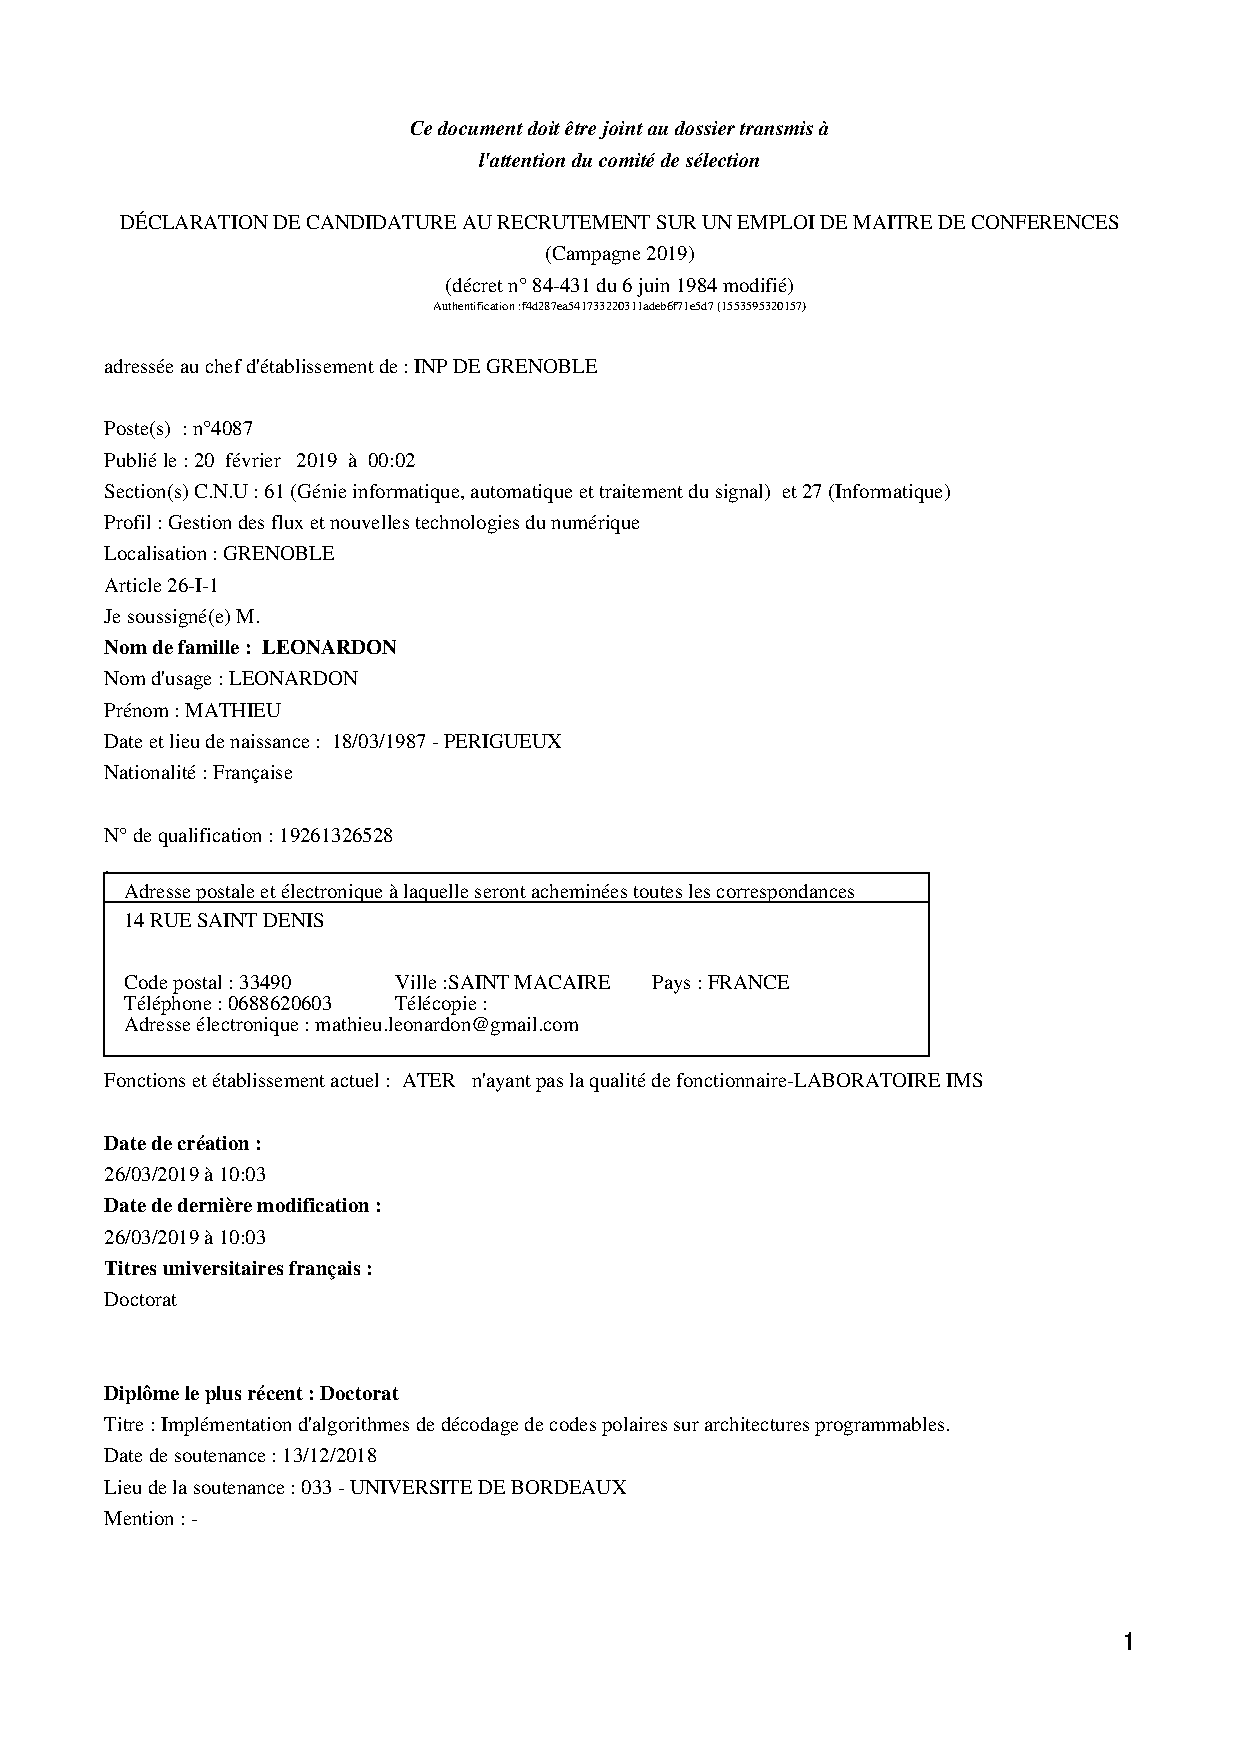
\includepdf[pages=1 , pagecommand={\section{D\'eclaration de candidature Galaxie}},width=\paperwidth, offset=80 -100]{candidatures/grenoble_inp}
    \includepdf[pages=2-,width=\paperwidth, offset=80 -100]{candidatures/grenoble_inp}
}{}
\ifthenelse{\equal{\version}{lyon_insa}}{
    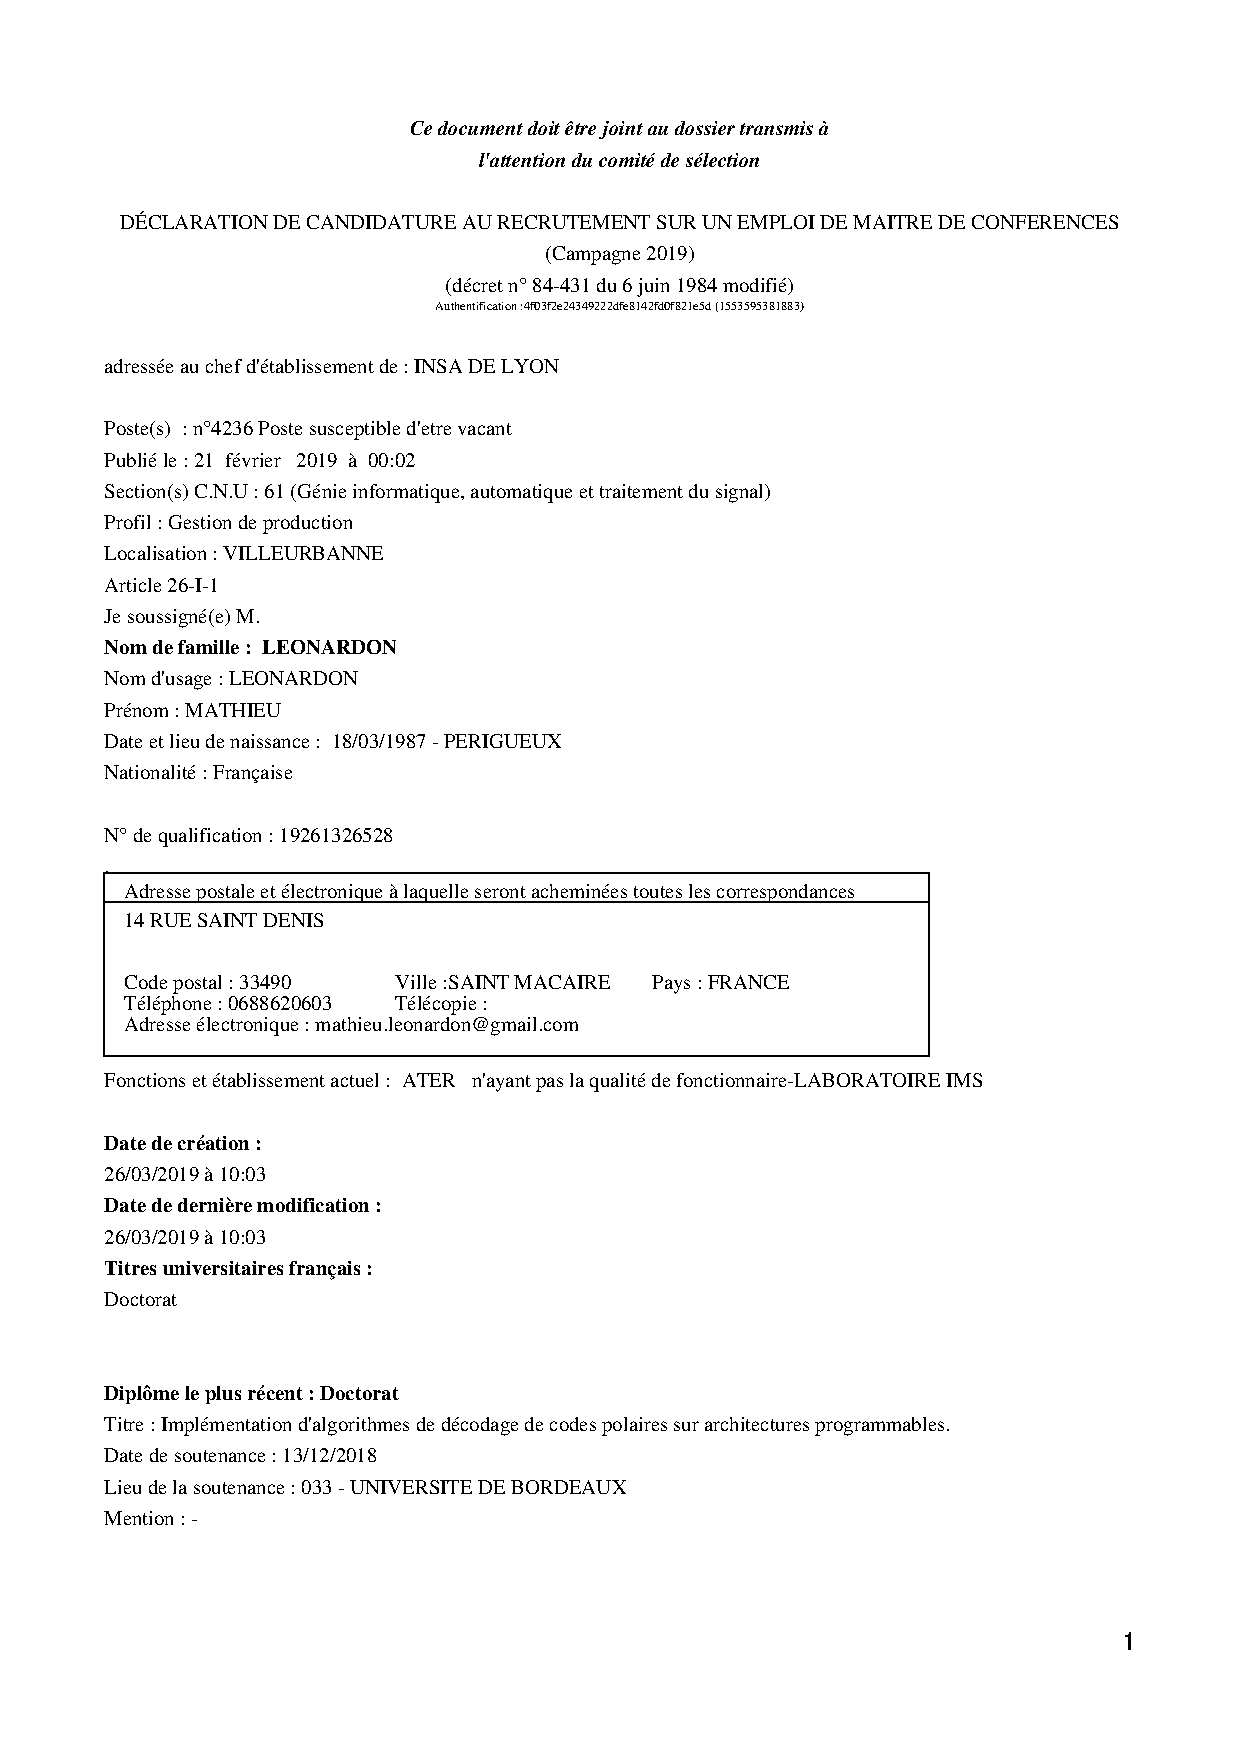
\includepdf[pages=1 , pagecommand={\section{D\'eclaration de candidature Galaxie}},width=\paperwidth, offset=80 -100]{candidatures/lyon_insa}
    \includepdf[pages=2-,width=\paperwidth, offset=80 -100]{candidatures/lyon_insa}
}{}
\ifthenelse{\equal{\version}{nantes_centrale}}{
    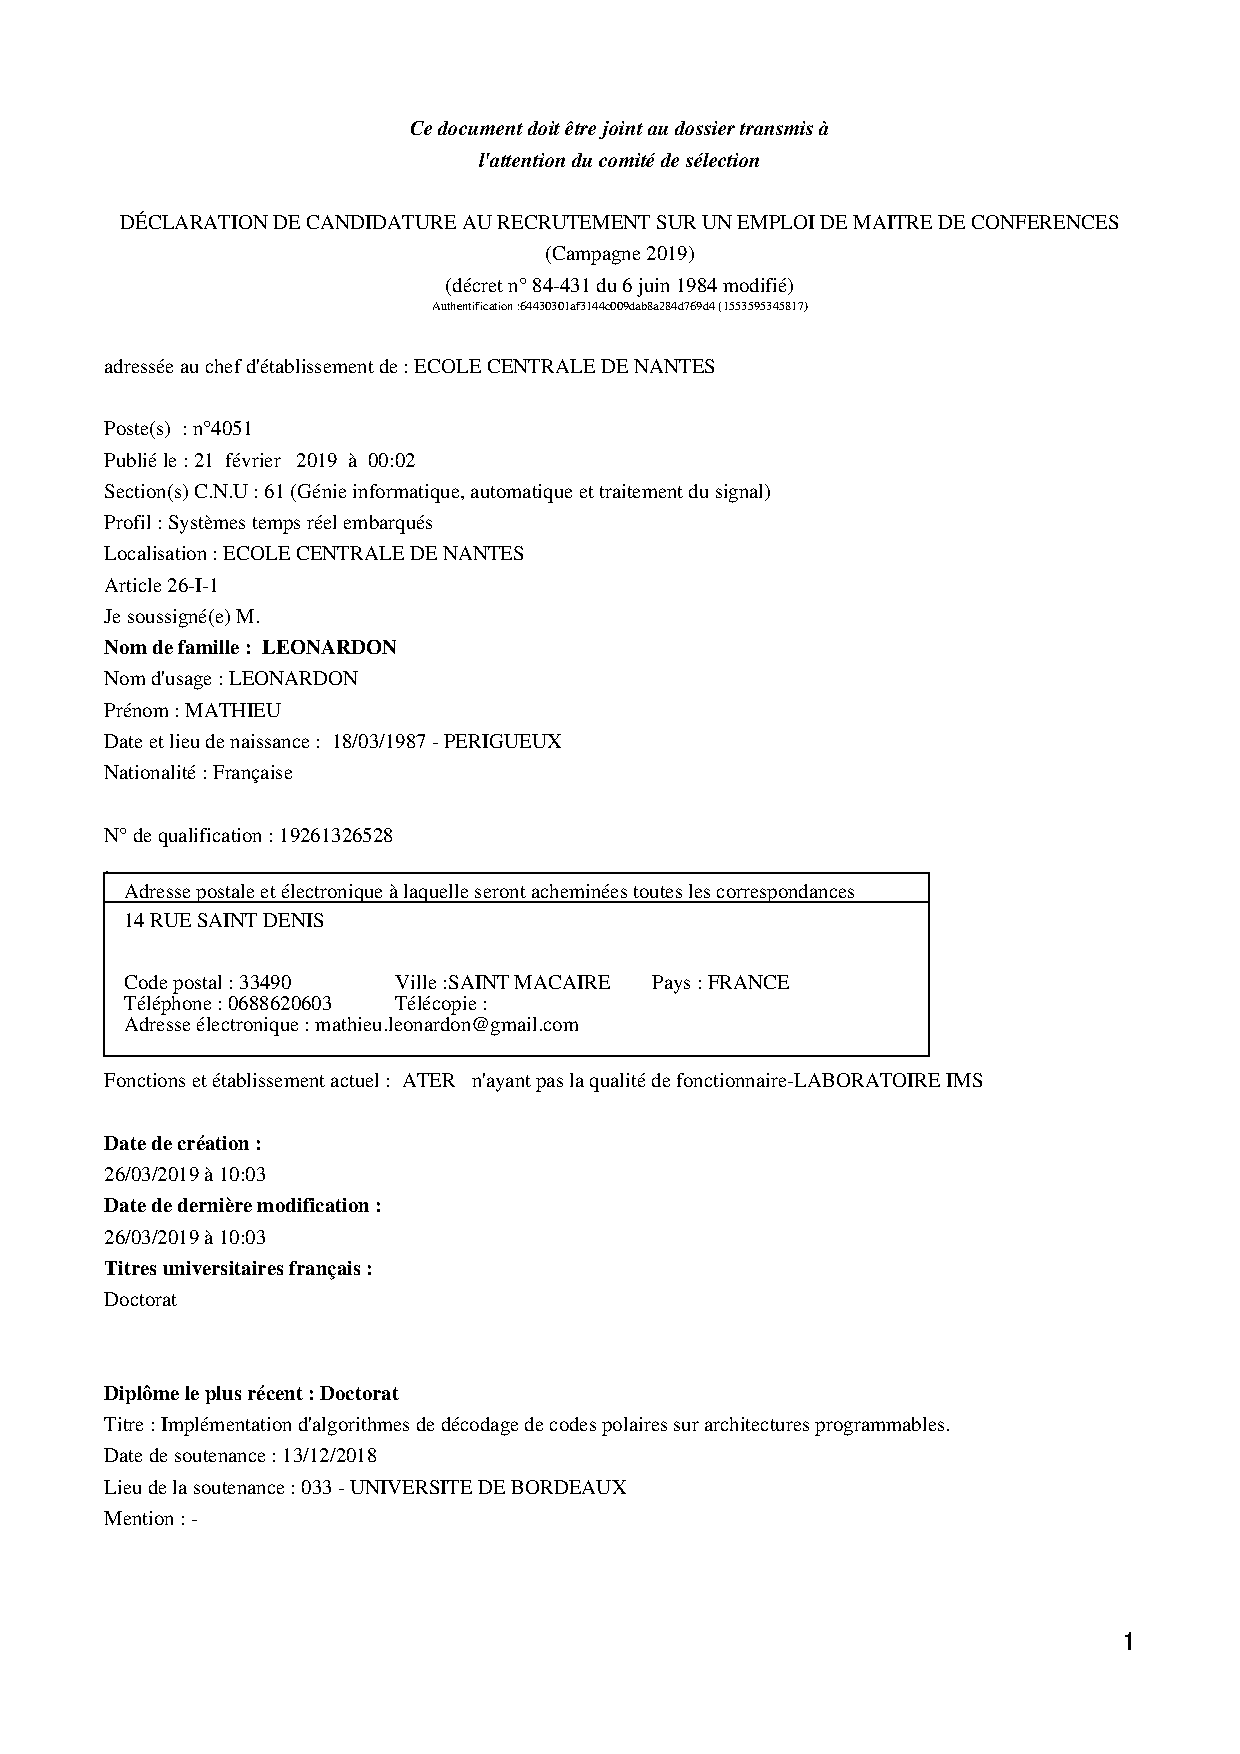
\includepdf[pages=1 , pagecommand={\section{D\'eclaration de candidature Galaxie}},width=\paperwidth, offset=80 -100]{candidatures/nantes_centrale}
    \includepdf[pages=2-,width=\paperwidth, offset=80 -100]{candidatures/nantes_centrale}
}{}
\ifthenelse{\equal{\version}{toulouse_inp}}{
    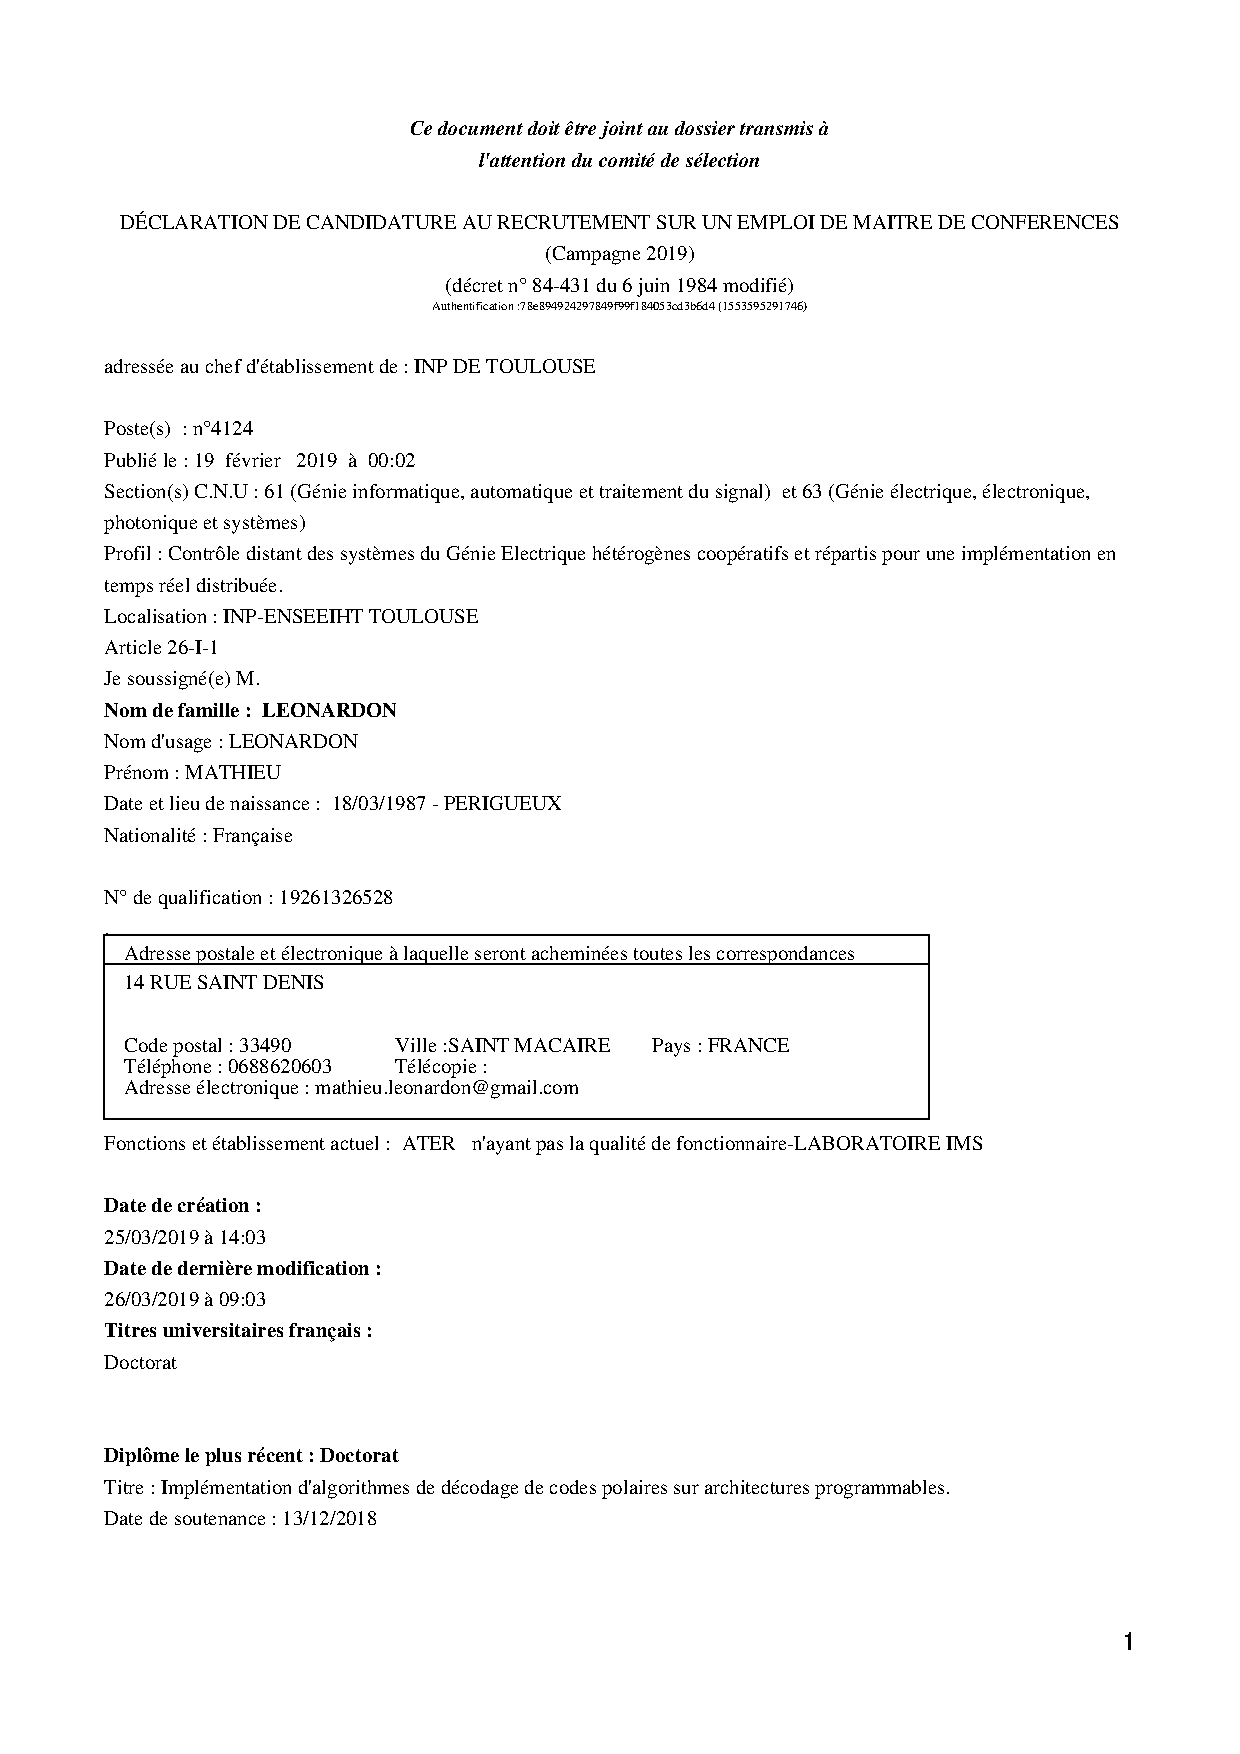
\includepdf[pages=1 , pagecommand={\section{D\'eclaration de candidature Galaxie}},width=\paperwidth, offset=80 -100]{candidatures/toulouse_inp}
    \includepdf[pages=2-,width=\paperwidth, offset=80 -100]{candidatures/toulouse_inp}
}{}
\ifthenelse{\equal{\version}{toulouse_insa}}{
    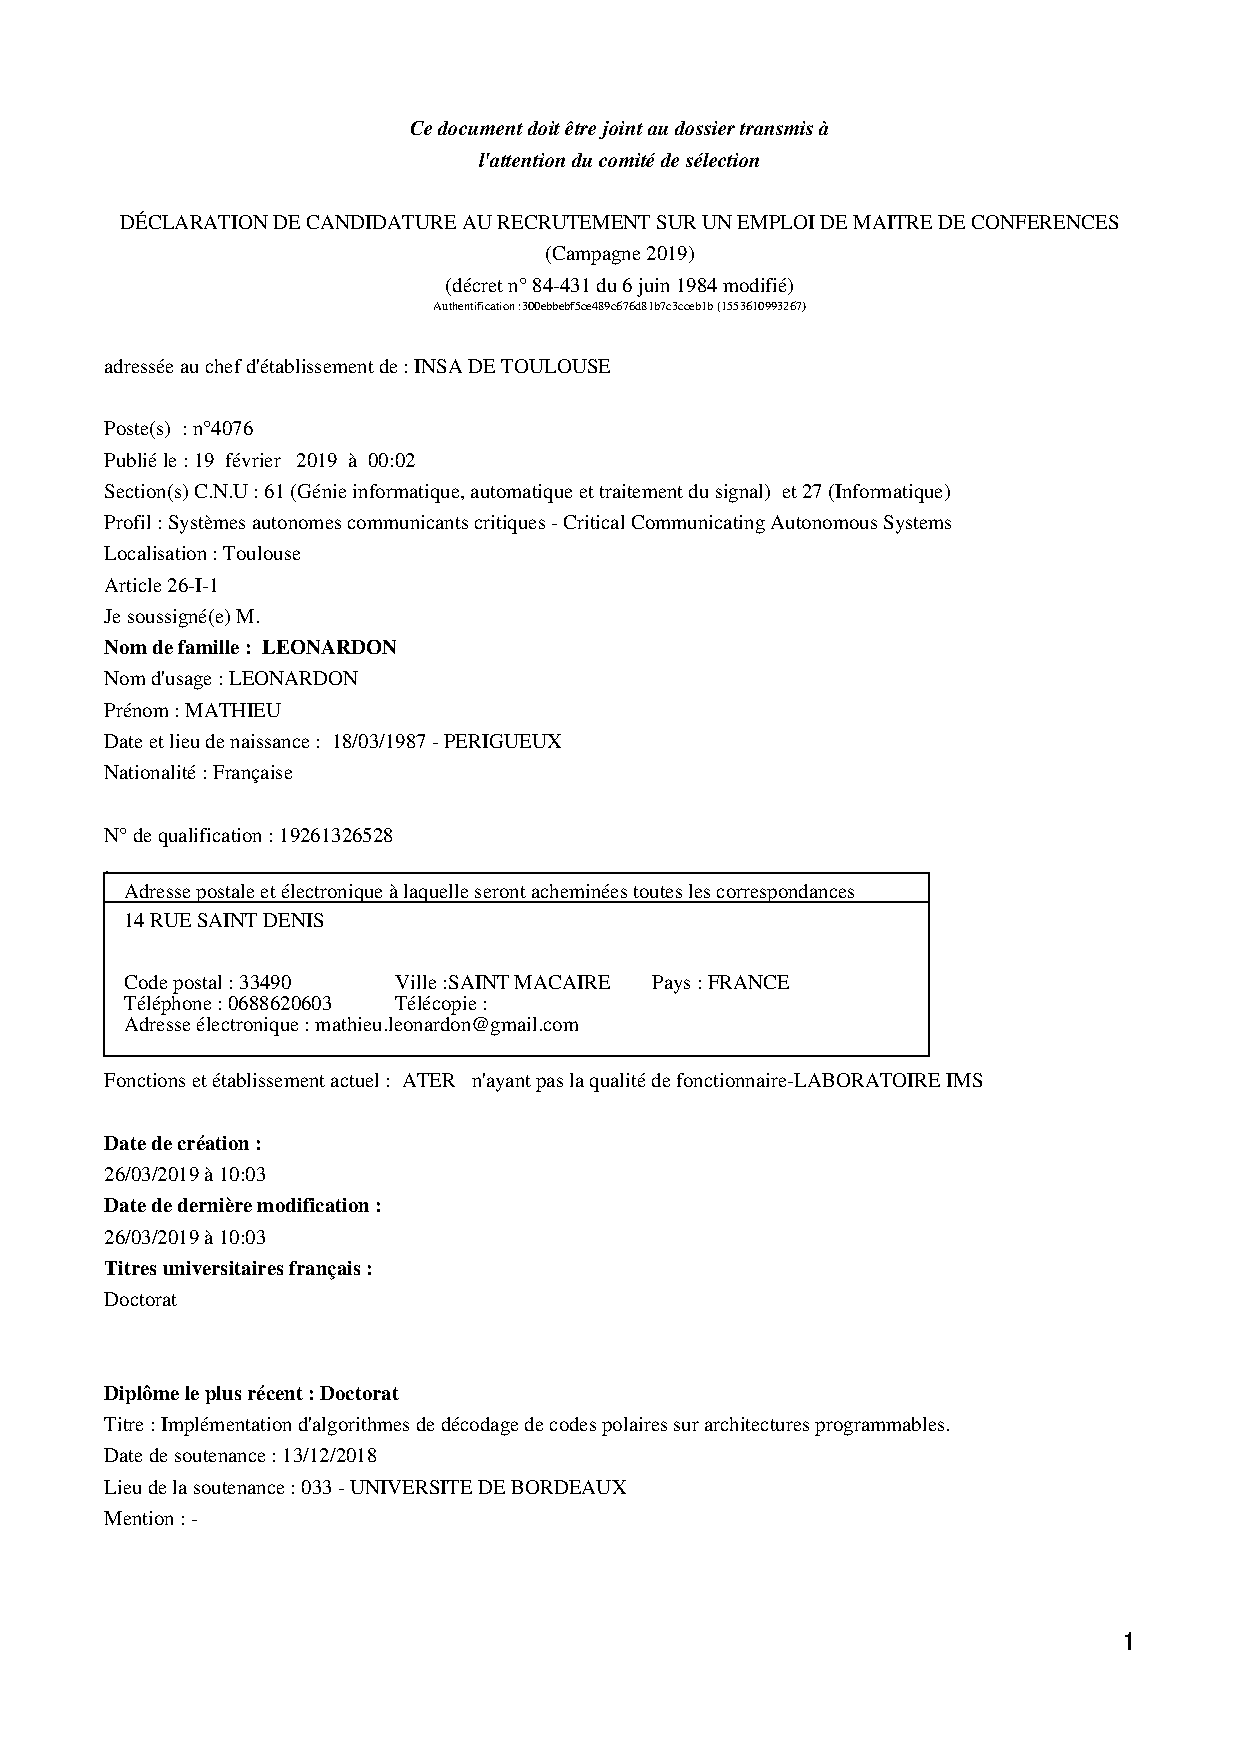
\includepdf[pages=1 , pagecommand={\section{D\'eclaration de candidature Galaxie}},width=\paperwidth, offset=80 -100]{candidatures/toulouse_insa}
    \includepdf[pages=2-,width=\paperwidth, offset=80 -100]{candidatures/toulouse_insa}
}{}

\newpage


\renewcommand{\tabcolsep}{0.1cm}
\renewcommand{\arraystretch}{1}

\definecolor{color0}{rgb}{0,0,0}% black
\definecolor{color1}{rgb}{0.22,0.45,0.70}% light blue
\definecolor{color2}{rgb}{0.45,0.45,0.45}% dark grey

\section{Curriculum Vitae d�taill�}
\begin{multicols}{2}\raggedright
\namestyle{Mathieu L�onardon} \\
\vspace{0.5cm}
\titlestyle{Docteur en \'Electronique}\\
\titlestyle{Qualifi� MCF sections 27, 61, 63}
\columnbreak

\raggedleft
\addressstyle{
14 rue Saint Denis \\
33490 Saint Macaire, France \\
e-mail : \url{mathieu.leonardon@gmail.com}\\
t�l : (+33)6 88 62 06 03\\
32 ans
}
\end{multicols}
\vspace{0.2cm}
\subsection{Activit� professionnelle actuelle}

\begin{flushleft}
\tabcv{2018 - 2019}{
\textbf{ATER}, \textit{Bordeaux INP}, \textit{laboratoire IMS}, \textit{Talence}\\[0.5em]
 {\footnotesize
 \textbf{$\bullet\ $Encadrants :} {Christophe J�go (IMS), Camille Leroux (IMS)}\\
\textbf{$\bullet\ $Sujet :} {Impl�mentations logicielles et mat�rielles d'algorithmes de d�codage de codes polaires}\\
\textbf{$\bullet\ $Enseignement :} {192 HETD de TP, TD et cours int�gr�s � l'ENSEIRB-MATMECA}
}
}

\subsection{Formation acad�mique}

\tabcv{2015 - 2018}{
\textbf{Doctorat en �lectronique en cotutelle}, \\ \textit{Universit� de Bordeaux}, \textit{laboratoire IMS}, \textit{France}, \\ \textit{Polytechnique Montr�al}, \textit{d�partement de G�nie \'Electrique}, \textit{Canada}\\[0.5em]
%\hbox{\phantom{\ \ \ \ }}\begin{minipage}{0.97\linewidth}
{\footnotesize \textbf{$\bullet\ $Sujet de th�se :} {D�codage de codes polaires sur des architectures programmables}\\
\textbf{$\bullet\ $Mots clefs :} {Codes polaires, d�codeur logiciel, ASIP, ad�quation algorithme-architecture}\\
\textbf{$\bullet$ Enseignement} : 45 HETD de TP, TD et cours int�gr�s � l'ENSEIRB-MATMECA\\
\textbf{$\bullet\ $Date de soutenance :} 13 d�cembre 2018\\
\textbf{$\bullet\ $Jury :} \\[0.25em]
\begin{tabular}{llll}
{Pr.} & {Mohamad Sawan}                    & {Polytechnique Montr�al} & {Pr�sident} \\
{Pr.} & {Amer Baghdadi}                    & {IMT Atlantique}         & {Rapporteur}\\
{Pr.} & {Emmanuel Casseau} \textbf{(S.61)} & {Universit� Rennes 1}    & {Rapporteur} \\
{Dr.} & {Olivier Muller}   \textbf{(S.63)} & {Grenoble INP}           & {Examinateur}\\
{Pr.} & {Charly Poulliat}  \textbf{(S.61)} & {INP Toulouse}           & {Examinateur}\\
{Dr.} & {Camille Leroux}   \textbf{(S.61)} & {Bordeaux INP}           & {Co-encadrant} \\
{Pr.} & {Christophe J�go}  \textbf{(S.61)} & {Bordeaux INP}           & {Directeur de th�se}\\
{Pr.} & {Yvon Savaria}                     & {Polytechnique Montr�al} & {Directeur de th�se}\\
\end{tabular}}
%\end{minipage}
}

\tabcv{2012 - 2015}{
\textbf{Dipl�me d'ing�nieur}, \textit{ENSEIRB-MATMECA}, \textit{Talence}\\[0.5em]
{\footnotesize \textbf{$\bullet$ Cursus :} Syst�mes \'Electroniques Embarqu�s (SEE)}, fili�re par apprentissage
}

\tabcv{2011 - 2012}{
\textbf{Dipl�me Universitaire de Technologie}, \textit{IUT Paul Sabatier}, \textit{Toulouse}\\[0.5em]
{\footnotesize\textbf{$\bullet$ Sp�cialit� :} Mesures Physiques }}

\subsection{Exp�riences professionnelles}

\tabcv{2012-2015}{
\textbf{Ing�nieur en apprentissage}, \textit{Worldcast Systems}, \textit{M�rignac}\\[0.5em]
{\footnotesize
\textbf{$\bullet$ Encadrant} : Herv� Garat\\
\textbf{$\bullet$ Sujet du m�moire} : Conception d'une interface homme-machine pour des �metteurs radio \\
\textbf{$\bullet$ Activit�s annexes} : Programmation microcontr�leur d'�metteurs FM

}
}

\tabcv{Juillet-Ao�t 2012}{
\textbf{Stagiaire}, \textit{I3S}, \textit{Laroque-d'Olmes}\\[0.5em]
{\footnotesize
\textbf{$\bullet$ Encadrants :} Nicolas Antini et Franck Dedieu\\
\textbf{$\bullet$ Sujet :} Conception d'une jauge �lectronique dot�e d'un afficheur pour mesure de niveau dans une cuve � l'aide d'un capteur de pression diff�rentielle
}
}

\end{flushleft}

\subsection{Liste des Publications}
{
\renewcommand{\refname}{\vspace{-2.5em}}

\nocite{*}
\begin{itemize}

\item \textbf{Manuscrit}
\newrefcontext[labelprefix=M]
\printbibliography[keyword={thesis}]
\vspace{2em}

\item \textbf{Journaux Internationaux}
\newrefcontext[labelprefix=IJ]
\printbibliography[keyword={journal}]
\vspace{2em}

\item \textbf{Conf�rences Internationales}
\newrefcontext[labelprefix=IC]
\printbibliography[keyword={international-conference}]
\vspace{2em}

\item \textbf{Conf�rences Nationales}
\newrefcontext[labelprefix=NC]
\printbibliography[keyword={national-conference}]
\vspace{2em}

\end{itemize}
}

\clearpage
\subsection{Activit�s d'enseignement}


\begin{center}
\begin{tabular}{|c|c|c|c|}
\hline
\textbf{�tablissement} & \textbf{Ann�e scolaire} & \textbf{Vol. horaire �q. TD} & \textbf{Section} \\ \hline \hline
{ENSEIRB-MATMECA} & {2015 - 2016} & {45 h} & 61 \\ \hline
{ENSEIRB-MATMECA} & {2018 - 2019} & {192 h} & 61 \\
\hline
\multicolumn{2}{c|}{} & 237 h �q. TD \\
\cline{3-3}
\end{tabular}
\end{center}
%\vspace{1em}


\subsubsection{Projet de conception en �lectronique}
\label{subsubsec:loto}
\begin{description}\parskip 0pt
\item[Responsable :] Mathieu L�onardon
\item[Niveau :] $1^{\mbox{�re}}$ ann�e ENSEIRB - Fili�re SEE- �quivalent Licence 3
\item[Volume :] 2 x 25 HETD
\item[Contenu :]  
La premi�re partie de ce module est un cours sur le flot de conception FPGA.
Les machines d'�tats sont �galement pr�sent�es et quelques exercices sont propos�s.
S'en suit un projet de conception d'une architecture num�rique. Les objectifs sont :
        \begin{itemize}
        \item concevoir une architecture mat�rielle,
        \item acqu�rir des comp�tence en VHDL,
        \item d�velopper un esprit synth�tique pour la r�daction du rapport,
        \item acqu�rir des comp�tences en pr�sentation de projet avec une soutenance.
    \end{itemize}
    
Le projet est la r�alisation d'un Loto sur une carte Nexys 4. L'utilisateur final doit pouvoir tirer 6 nombres al�atoirement, sans retirage. Ces nombres sont affich�s sur des afficheurs 7 segments.
\item[Mots-cl�s :] FPGA, VHDL, Electronique num�rique 
\item[Participation personnelle :] Cours int�gr�, encadrement du projet. 
\item[Ressources p�dagogiques cr��es :] \url{https://bit.ly/2HLfaXt}
\end{description}


\subsubsection{Architecture reconfigurable}
\label{subsubsec:reconf}
\begin{description}\parskip 0pt
\item[Responsable :]  Mathieu L�onardon
%\item[Effectif :] Environ 15 �l�ves
\item[Niveau :] $2^{\mbox{�me}}$ ann�e ENSEIRB-MATMECA - Fili�re SEE - �quivalent Master 1
\item[Volume :] 1 x 20 HETD
\item[Contenu :] Conception avanc�e sur les circuits FPGA. Objectifs :
    \begin{itemize}
        \item d�finir les architectures reconfigurables,
        \item comprendre leur structure interne,
        \item comprendre leur fonctionnement,
        \item mise en oeuvre de techniques avanc�es,
        \item acqu�rir des comp�tences en pr�sentation de projet avec une petite soutenance.
    \end{itemize}
\item[Mots-cl�s :] FPGA, VHDL, Electronique num�rique 
\item[Participation personnelle :] Cours int�gr�, encadrement d'un projet.
\item[Ressources p�dagogiques cr��es :] \url{https://bit.ly/2U4Ua4o }
\end{description}

\subsubsection{�lectronique Num�rique}
\label{subsubsec:rsi}
\begin{description}\parskip 0pt
\item[Responsable :] Mathieu L�onardon
%\item[Effectif :] Environ 15 �l�ves
\item[Niveau :] $1^{\mbox{�re}}$ ann�e ENSEIRB-MATMECA - Fili�re RSI- �quivalent Licence 3
\item[Volume :] 1 x 25 HETD
\item[Contenu :] Ce module pr�sente les notions de bases de l'�lectronique num�rique : la num�ration, l'alg�bre de Boole, la logique combinatoire ainsi que la logique s�quentielle. Architecture et fonctionnement d'une machine � �tats finis. Bases de technologie des circuits imprim�s.
\item[Mots-cl�s :] Num�ration, Machine � �tats finis, technologie CMOS, Electronique num�rique 
\item[Participation personnelle :] Cours int�gr� - TD
\item[Ressources p�dagogiques cr��es :] \url{https://bit.ly/2U0hgsV}
\end{description}


\subsubsection{Logique combinatoire et logique s�quentielle}
\label{subsubsec:en1}
\begin{description}\parskip 0pt
\item[Responsable :] Christophe J�go
%\item[Effectif :] Environ 15 �l�ves
\item[Niveau :] $1^{\mbox{�re}}$ ann�e ENSEIRB-MATMECA - Fili�re �lectronique- �quivalent Licence 3
\item[Volume :] 1 x 32 HETD
\item[Contenu :] ~

\begin{itemize}
\item Les fonctions �l�mentaires combinatoires et s�quentielles utilis�es dans les circuits num�riques,
\item la mod�lisation des fonctions num�riques � l'aide du langage VHDL.
\end{itemize}
A l'issue du cours, l'�tudiant doit �tre capable :
\begin{itemize} 
\item de d�crire une fonction combinatoire et la repr�senter par un circuit num�rique,
\item de d�crire et synth�tiser un compteur, une machine � �tats,
\item de rep�rer le chemin critique d'une fonction logique complexe et de calculer sa fr�quence maximale de fonctionnement.
\end{itemize}
Six s�ances de travaux dirig�s de quatre heures compl�tes le cours. Chaque s�ance se d�compose en deux parties. 
Des th�mes sont trait�s dans une premi�re partie. 
Dans une seconde partie, les syst�mes num�riques d�finis sont d�crits dans le langage de description mat�riel VHDL. 
Cette approche permet d'initier progressivement les �tudiants � ce langage. 
\item[Mots-cl�s :] Electronique num�rique, VHDL, FPGA
\item[Participation personnelle :] Encadrement des TP et du projet
\end{description}

\noindent \subsubsection{Projet micro-processeur}
\begin{description}\parskip 0pt
\item[Responsable :] Val�ry Lebret
\item[Niveau :] $1^{\mbox{�re}}$ ann�e ENSEIRB-MATMECA - Fili�re �lectronique- �quivalent Licence 3
\item[Volume :] 1 x 36 HETD
\item[Contenu :] Cet enseignement a pour objectif la programmation de microcontr�leurs PIC de MICROCHIP, choisis pour leur facilit� de mise en oeuvre li� � leur faible complexit�. 
Apr�s une pr�sentation de cette famille de microcontr�leurs et de leurs sp�cificit�s, l'activit� commence par l'�criture de programmes simples en langage assembleur visant � illustrer le fonctionnement du microcontr�leur (codage et ex�cution des instructions, acc�s aux registres, gestions des ressources internes et des entr�es/sorties...). 
Une carte d'application int�grant un PIC16F84 sert de support, le d�veloppement logiciel se faisant gr�ce � la chaine d'outils int�gr�s MPLABX qui dispose notamment d'un simulateur. 
La programmation s'effectue ensuite en langage C avec pour finalit� la mise en oeuvre d'un projet (par exemple une horloge � quartz sur afficheur LCD) au moyen de la carte de d�veloppement PICDEM2 comportant une cible PIC16F877 (plus de ressources internes, possibilit� de faire du d�bogage). L'accent est mis sur les limitations rencontr�es sur les syst�mes embarqu�s lors de la programmation en langage C (espace m�moire r�duit, puissance de calcul limit�e, ..) ainsi que sur la gestion des interruptions.
\item[Mots-cl�s :] Programmation microcontr�leur, langage assembleur
\item[Participation personnelle :] Encadrement des TP
\end{description}


\noindent \subsubsection{Architecture des ordinateurs}
\begin{description}\parskip 0pt
\item[Responsable :] J�r�mie Crenne
\item[Niveau :] $2^{\mbox{�me}}$ ann�e ENSEIRB-MATMECA - Fili�re �lectronique- �quivalent Master 1
\item[Volume :] 1 x 16 HETD
\item[Contenu :] Cet enseignement a pour but de renforcer les connaissances en abordant des techniques plus avanc�es relatives aux processeurs et aux m�moires. Ce cours est articul� autour du livre de J.L. Hennessy et A. Patterson "Computer Architecture, a quantitative approach". Sont abord�s les architectures RISC et CISC, les architecture pipeline, les al�as de donn�es et de contr�le. Le cas du processeur MIPS est �tudi� en d�tail pour donner aux �tudiants un exemple concret d'architecture de processeur.
La finalit� de ce cours est de permettre aux �tudiants de comprendre les syst�mes multi/many-coeurs les plus sophistiqu�s.
\item[Mots-cl�s :] Architecture des ordinateurs, architectures pipelines, multifil
\item[Participation personnelle :] Encadrement des TD
\end{description}

\noindent \subsubsection{Projet micro-informatique}
\begin{description}\parskip 0pt
\item[Responsable :] Yannick Bornat
\item[Niveau :] $2^{\mbox{�me}}$ ann�e ENSEIRB-MATMECA - Fili�re �lectronique- �quivalent Master 1
\item[Volume :] 1 x 42 HETD
\item[Contenu :] 
L'ensemble de TPs s'effectue sur microcontr�leur AT91SAM7X256. Ce microcontr�leur poss�de un coeur ARM7, de nombreux p�riph�riques ainsi qu'un syst�me d'interruptions vectoris�es et param�trable.
L'objectif de l'enseignement est d'utiliser les diff�rentes ressources mat�rielles pour concevoir un syst�me d'exploitation minimaliste couvrant les besoins sp�cifiques des microcontr�leurs pour des t�ches temps r�el.
Les notions abord�es couvrent les aspects temps-r�el, communication, int�grit� des donn�es.
Les �tudiants sont plac�s dans une situation o� leur seul source de documentation est constitu�e par les documents techniques constructeur en anglais.

\item[Mots-cl�s :] Programmation microcontr�leur, langage C, r�seaux d'interruptions
\item[Participation personnelle :] Encadrement des TP et du projet
\end{description}

\noindent \subsubsection{Programmation objet. Langage C++}
\begin{description}\parskip 0pt
\item[Responsable :] Bertrand Le Gal
\item[Niveau :] $2^{\mbox{�me}}$ ann�e ENSEIRB-MATMECA - Fili�re �lectronique- �quivalent Master 1
\item[Volume :] 1 x 15 HETD
\item[Contenu :] 
Cet enseignement vise � apporter aux �tudiants les base de la programmation orient�e objets. Les concepts g�n�raux de la programmation orient�e objets sont introduits en cours. Le langage C++ est utilis� afin d'illustrer les concepts manipul�s. L'ensemble de ces notions sont mises � profit dans un projet afin d'illustrer de mani�re pratique l'interet de cette approche de programmation.
\item[Mots-cl�s :] Programmation orient�e objet, C++
\item[Participation personnelle :] Encadrement des TP
\end{description}

\clearpage
%###################


\subsection{Activit�s de recherche}
\label{subsec:rech}
L'ensemble des travaux pr�sent�s ici ont �t� r�alis�s durant mes trois ann�es de doctorat.

\subsubsection{Les codes polaires}

La th�matique principale de ma th�se concernait le d�codage de codes polaires. Les codes polaires constituent une classe de codes correcteurs d'erreurs invent�e r�cemment qui suscite l'int�r�t des chercheurs et des industriels, comme en atteste leur s�lection pour le codage des canaux de contr\^ole dans la prochaine g�n�ration de t�l�phonie mobile (5G). Un des enjeux des futurs r�seaux mobiles est la virtualisation des traitements num�riques du signal, et en particulier les algorithmes de codage et de d�codage.  Afin d'am�liorer la flexibilit� du r�seau, ces algorithmes doivent �tre d�crits de mani�re logicielle et �tre d�ploy�s sur des architectures programmables. Une telle infrastructure  de r�seau permet de mieux r�partir l'effort de calcul sur l'ensemble des n\oe{}uds et d'am�liorer la coop�ration entre cellules. Ces techniques ont pour but de r�duire la consommation d'�nergie, d'augmenter le d�bit et de diminuer la latence des communications. Les travaux pr�sent�s dans le manuscrit de th�se ont port� sur l'impl�mentation logicielle des algorithmes de d�codage de codes polaires et la conception d'architectures programmables sp�cialis�es pour leur ex�cution.

\subsubsection{Impl�mentation logicielle d'algorithmes de d�codage de codes polaires sur processeurs g�n�ralistes}
% R�organiser : pas clair
Une des caract�ristiques principales d'une cha�ne de communication mobile est l'instabilit� du canal de communication. Afin de rem�dier � cette instabilit�, des techniques de modulations et de codages adaptatifs sont utilis�es dans les normes de communication. Ces techniques impliquent que les d�codeurs supportent une vaste gamme de codes : ils doivent �tre g�n�riques. La premi�re contribution de ces travaux est l'impl�mentation logicielle de d�codeurs g�n�riques des algorithmes de d�codage \og � Liste \fg (SCL : Successive Cancellation List) sur des processeurs � usage g�n�ral \cite{leonardon_2019}. Les unit�s SIMD pr�sentes sur les processeurs modernes permettent d'exploiter le parall�lisme disponible dans les algorithmes de d�codage de codes polaires.

Cette premi�re contribution a impliqu� la d�finition de deux concepts distincts : la g�n�ricit� et la flexibilit� d'un d�codeur de codes polaires. La flexibilit�, d'une part, est la capacit� d'un d�codeur � s'adapter � un standard de communications. En effet, les param�tres que sont la taille d'une trame, le nombre de bits d'information, la concat�nation d'un code CRC, la capacit� � g�rer des sch�mas de poin�onnage, sont des �l�ments d�finis par le standard. Un d�codeur g�n�rique doit �tre capable de supporter cette g�n�ricit� vis-�-vis du sch�ma d'encodage. D'autre part, la flexibilit� d'un d�codeur de codes polaires correspond � la possibilit� d'ajuster l'algorithme et l'impl�mentation du d�codeur afin de proposer des compromis entre d�bit et latence, pour un m�me sch�ma d'encodage. Les param�tres qui concernent la flexibilit� sont par exemple la profondeur de la liste pour les algorithmes SCL, le format de repr�sentation des entiers (quantification) ou encore la gestion de variantes algorithmiques adaptatives de l'algorithme SCL.
Le d�codeur propos� s'attache � �tre le plus g�n�rique et le plus flexible possible. La g�n�ricit� et la flexibilit� du d�codeur propos� sont sup�rieures � toutes les impl�mentations de l'�tat de l'art en ce qui concerne les algorithmes de d�codage � liste, qui sont les algorithmes pr�sentant les meilleures performances de d�codage.
% D�tailler flexibilit� (quantification, variantes adaptatives, profondeur de la liste)
De plus, des am�liorations algorithmiques et d'impl�mentations sont propos�es, permettant d'augmenter les performances de d�bits et de latence de d�codage. Malgr� une g�n�ricit� et une flexibilit� accrue, les d�bits de d�codage atteints sont sup�rieurs (jusqu'� un facteur 5) � ceux de la litt�rature. Une version des d�codeurs propos�e a �galement �t� port�e sur ARM. Elle utilise le jeu d'instructions SIMD NEON. Si des d�bits inf�rieurs sont atteints, il est montr� que la consommation �nerg�tique sur ARM est r�duite en comparaison avec les impl�mentations sur les processeurs d'architecture x86.
Les d�codeurs sont tous int�gr�s � la suite logicielle AFF3CT (\url{aff3ct.github.io}). Le code source est donc mis � disposition de la communaut� scientifique et les r�sultats facilement reproductibles.

\subsubsection{D�codeur ASIP de codes polaires : sp�cialisation d'un processeur de base}


La deuxi�me contribution de mes travaux de th�se est la proposition d'une nouvelle architecture programmable performante sp�cialis�e dans le d�codage de codes polaires \cite{Leonardon2018a}. 
Elle d�coule de l'observation suivante : si les d�bits atteints par les d�codeurs logiciels sont �lev�s, surtout lorsque l'on consid�re des architectures multic\oe{}urs, leur point faible est leur consommation �nerg�tique. D�s lors, la probl�matique est d'identifier des architectures pouvant conserver une grande flexibilit� tout en �tant plus efficaces �nerg�tiquement. La famille des processeurs � jeu d'instructions d�di�s � l'application (ASIP : Application Specific Instruction set Processor) est une solution efficace et �l�gante.

L'approche que nous avons tout d'abord choisie est celle propos�e par les outils de Cadence / Tensilica. Un processeur de type RISC � faible constitue la base des processeurs XTensa. Cette base peut �tre configur�e. Nous avons donc �limin� le superflu (unit�s de calculs en virgule flottante, acc�l�rateurs mat�riels pour la multiplication) et ajout� du parall�lisme d'instructions (VLIW : Very Large Instruction Word). Le jeu d'instructions des processeurs XTensa peut �galement �tre enrichi, conjointement � la d�finition d'unit�s mat�rielles sp�cialis�es dans l'application qui nous int�resse, c'est-�-dire le d�codage de codes polaires.
Un des avantages de cette solution est que l'algorithme est d�fini de mani�re logicielle, permettant ainsi un d�veloppement rapide.

Les m�triques de consommation et d'surface occup�e sont alors g�n�r�es par l'outil. Un simulateur permet d'ex�cuter l'algorithme et de mesurer ainsi le nombre de cycles n�cessaire au d�codage des trames. Les r�sultats obtenus montrent que cette architecture atteint des d�bits et des latences proches des impl�mentations logicielles de l'�tat de l'art sur des processeurs � usage g�n�ral. La consommation �nerg�tique est r�duite d'un ordre de grandeur. En effet, lorsque l'on consid�re le d�codage par annulation successive d'un code polaire (1024,512), l'�nergie n�cessaire par bit d�cod� est de l'ordre de 10 nJ sur des processeurs � usage g�n�ral contre 1 nJ sur le processeur propos�s.

\subsubsection{D�codeur ASIP de codes polaires : description compl�te de l'architecture}
La troisi�me contribution de mes travaux de th�se est �galement une architecture de processeur � jeu d'instructions d�di� � l'application. Elle r�pond � la m�me probl�matique : proposer une impl�mentation flexible en augmentant les performances de d�bit, latence et consommation �nerg�tique. Elle se diff�rencie de la pr�c�dente par l'utilisation d'une m�thodologie de conception alternative. Au lieu d'�tre bas�e sur une architecture de type RISC, l'architecture du processeur propos� fait partie de la classe des architectures d�clench�es par le transfert de donn�es (TTA : Transport Triggered Architectures). Ces architectures sont constitu�es d'unit�s fonctionnelles r�alisant les op�rations sur les donn�es (chargement, sauvegarde, calcul) et de bus de transport les reliant. Dans une architecture de processeur classique, le contenu de l'instruction est l'op�ration � r�aliser accompagn�e des adresses des donn�es d'entr�e et de sortie. Dans les architectures TTA, chaque bus se voit attribuer une instruction durant chaque cycle. Chaque instruction contient un port de source et un port de destination. On parle de chemin de donn�e expos� : le programmeur (ou le compilateur) peut sp�cifier le chemin de donn�e de chaque instruction. Cette propri�t� permet des optimisations fines de l'impl�mentation d'un algorithme.

Une suite d'outils de d�veloppement libre est propos�e par l'universit� de Tampere (\url{http://openasip.org/}). Cette derni�re permet d'automatiser une grande partie de la conception d'un tel processeur et propose �galement un compilateur qui s'adapte � l'architecture sp�cialis�e. Ainsi, tout comme l'ASIP pr�c�dent, l'algorithme de d�codage est d�crit � l'aide d'un langage de haut niveau. Le d�codeur de codes polaires d'architecture TTA r�alis� a �t� prototyp� sur FPGA et sa synth�se a �t� r�alis� pour une cible ASIC dans la technologie ST FD-SOI 28 nm \cite{Leonardon2018b}. Les d�bits mesur�s sont alors sup�rieurs � ceux obtenus sur les processeurs � usage g�n�ral. La consommation �nerg�tique est r�duite � environ 0.1 nJ par bit d�cod� pour un code polaire (1024,512) avec l'algorithme de d�codage par annulation successive. Cela correspond � une r�duction de deux ordres de grandeur en comparaison de la consommation mesur�e sur des processeurs � usage g�n�ral, et � une r�duction d'un ordre de grandeur en comparaison avec l'ASIP r�alis� � l'aide des outils Cadence / Tensilica.

\subsubsection{Travaux sur le d�codeur Sparse Code Multiple Access}

Lors de mon s�jour � Polytechnique Montr�al, dans le cadre de mes travaux de th�se, je me suis int�ress� � l'impl�mentation d'un d�codeur SCMA (Sparse Code Multiple Access). SCMA est une technique d'acc�s multiple non orthogonal prometteuse pour les futures normes de communication. Alirezah Ghaffari a propos� des simplifications calculatoires de l'algorithme afin d'acc�l�rer le traitement de d�codage. Afin de s'assurer des performances r�elles de cette simplification, nous avons int�gr� ce d�codeur SCMA dans une cha�ne de communication compl�te. Il est �galement int�gr� dans AFF3CT pour rendre le code source disponible � la communaut� et �galement permettre donc la reproduction des r�sultats. Ces travaux sont d�crits dans \cite{Ghaffari2017}. Dans un second temps, nous nous sommes int�ress�s � l'acc�l�ration de l'impl�mentation logicielle de ces algorithmes sur processeurs g�n�raliste, par l'utilisation de jeu d'instructions SIMD \cite{ghaffari_2019}. L'utilisation des unit�s SIMD conjointement aux simplifications propos�es permet des gains en d�bit et en consommation �nerg�tique importants, jusqu'� un ordre de grandeur.

\subsubsection{Contribution au projet AFF3CT}
Je contribue depuis 2015 au d�veloppement du projet AFF3CT (\url{aff3ct.github.io}). Il s'agit d'un projet proposant de nombreux outils logiciels en lien avec les communications num�riques. Une attention particuli�re est port�e sur les performances en d�bit et en latence des d�codeurs de codes correcteurs d'erreurs. 

Utilis� comme simulateur, il permet de r�aliser des simulations de type Monte Carlo de l'ensemble de la cha�ne de communication. Les donn�es sont g�n�r�es al�atoirement, encod�es, modul�es, bruit�es, d�cod�es, et les performances sont estim�es en mesurant le taux d'erreur binaire (BER : Bit Error Rate) et le taux d'erreur trame (FER : Frame Error Rate). L'ambition du simulateur est triple : 
\begin{enumerate}
    \item \textbf{Reproductibilit�} : il est souvent difficile de reproduire les r�sultats de la litt�rature. Beaucoup de param�tres peuvent �tre omis, qui emp�chent une reproduction fid�le des algorithmes propos�s. C'est pourquoi une large base de donn�es de courbes pr�-simul�es avec l'ensemble des param�tres n�cessaires est disponible. D�s lors, de nombreux projets de recherche utilisent AFF3CT comme r�f�rence. \'Etant open-source, les descriptions logicielles sont accessibles par tous.
    \item \textbf{Simulations haut d�bit} : afin d'estimer correctement des BER / FER, il est n�cessaire de simuler une centaine de trames erron�es pour une valeur de rapport signal � bruit. Lorsque le FER � simuler est bas, par exemple $10^{-7}$, environ 1 milliard de trames doivent �tre simul�es. Lorsque les trames sont de grande taille les temps de simulation peuvent s'av�rer extr�mement longs. Il est donc tr�s utile de disposer de simulations haut d�bit. C'est pour cette raison que nous utilisons tout le parall�lisme disponible : parall�lisme de donn�es, par l'utilisation d'instructions SIMD, parall�lisme d'instructions, avec l'utilisation des architectures superscalaires et multic\oe{}urs, et enfin l'utilisation de n\oe{}uds multiples est assur�e gr�ce � la librairie \texttt{openmpi}. Ceci permet d'atteindre des d�bits tr�s importants. Par exemple, 63 Gbps sont atteints pour le d�codeur FA-SCL pr�sent� dans \cite{leonardon_2019} sur le n\oe{}ud miriel de la plateforme PLAFRIM (\url{https://www.plafrim.fr/en/the-platform/hardware-documentation/}).
    \item \textbf{H�t�rog�n�it� des algorithmes} : dans le domaine des d�codeurs de codes correcteurs d'erreurs, il existe de tr�s nombreux algorithmes de d�codage. Effectuer une comparaison exhaustive avec l'existant est donc souvent tr�s difficile. L'ambition d'AFF3CT est de couvrir le maximum de variantes algorithmiques de la litt�rature pour faciliter le travail des chercheurs.
\end{enumerate}

AFF3CT peut �galement �tre utilis� en tant que librairie. Ainsi, n'importe quel d�veloppeur peut utiliser les briques �l�mentaires disponibles. Cette possibilit� est beaucoup utilis� par nos partenaires industriels (Airbus, Thales, ...) pour int�grer les blocs d'AFF3CT � leurs cha�nes de communication, que ce soit pour de la simulation ou pour des syst�mes communicants r�els (radio logicielle).
\clearpage

\subsection{Responsabilit�s collectives}
Je suis membre IEEE depuis 2018 et je participe � la relecture d'articles pour diff�rentes revues et conf�rences dans le domaine des syst�mes num�riques et du traitement du signal.
\subsubsection{Revue d'articles de journaux}
\begin{itemize}
    \item IEEE Communication Letters
\end{itemize}

\subsubsection{Revue d'articles de conf�rence}
\begin{itemize}
    \item IEEE International Symposium on Information Theory : ISIT
    \item IEEE Wireless Communications and Networking Conference : WCNC
    \item IEEE International Conference on Communications : ICC
    \item IEEE Workshop on Signal Processing Systems : SiPS
\end{itemize}

\subsubsection{CCT TSI CNES}
En juin 2015, j'ai particip� � la journ�e \og Technologies pour la 5G - segment spatial \fg organis�e par le CNES � Toulouse, pour une pr�sentation nomm�e \og Les codes polaires, algorithmes et d�codeurs \fg, durant laquelle j'ai pu �changer avec les diff�rents intervenants. 

\clearpage


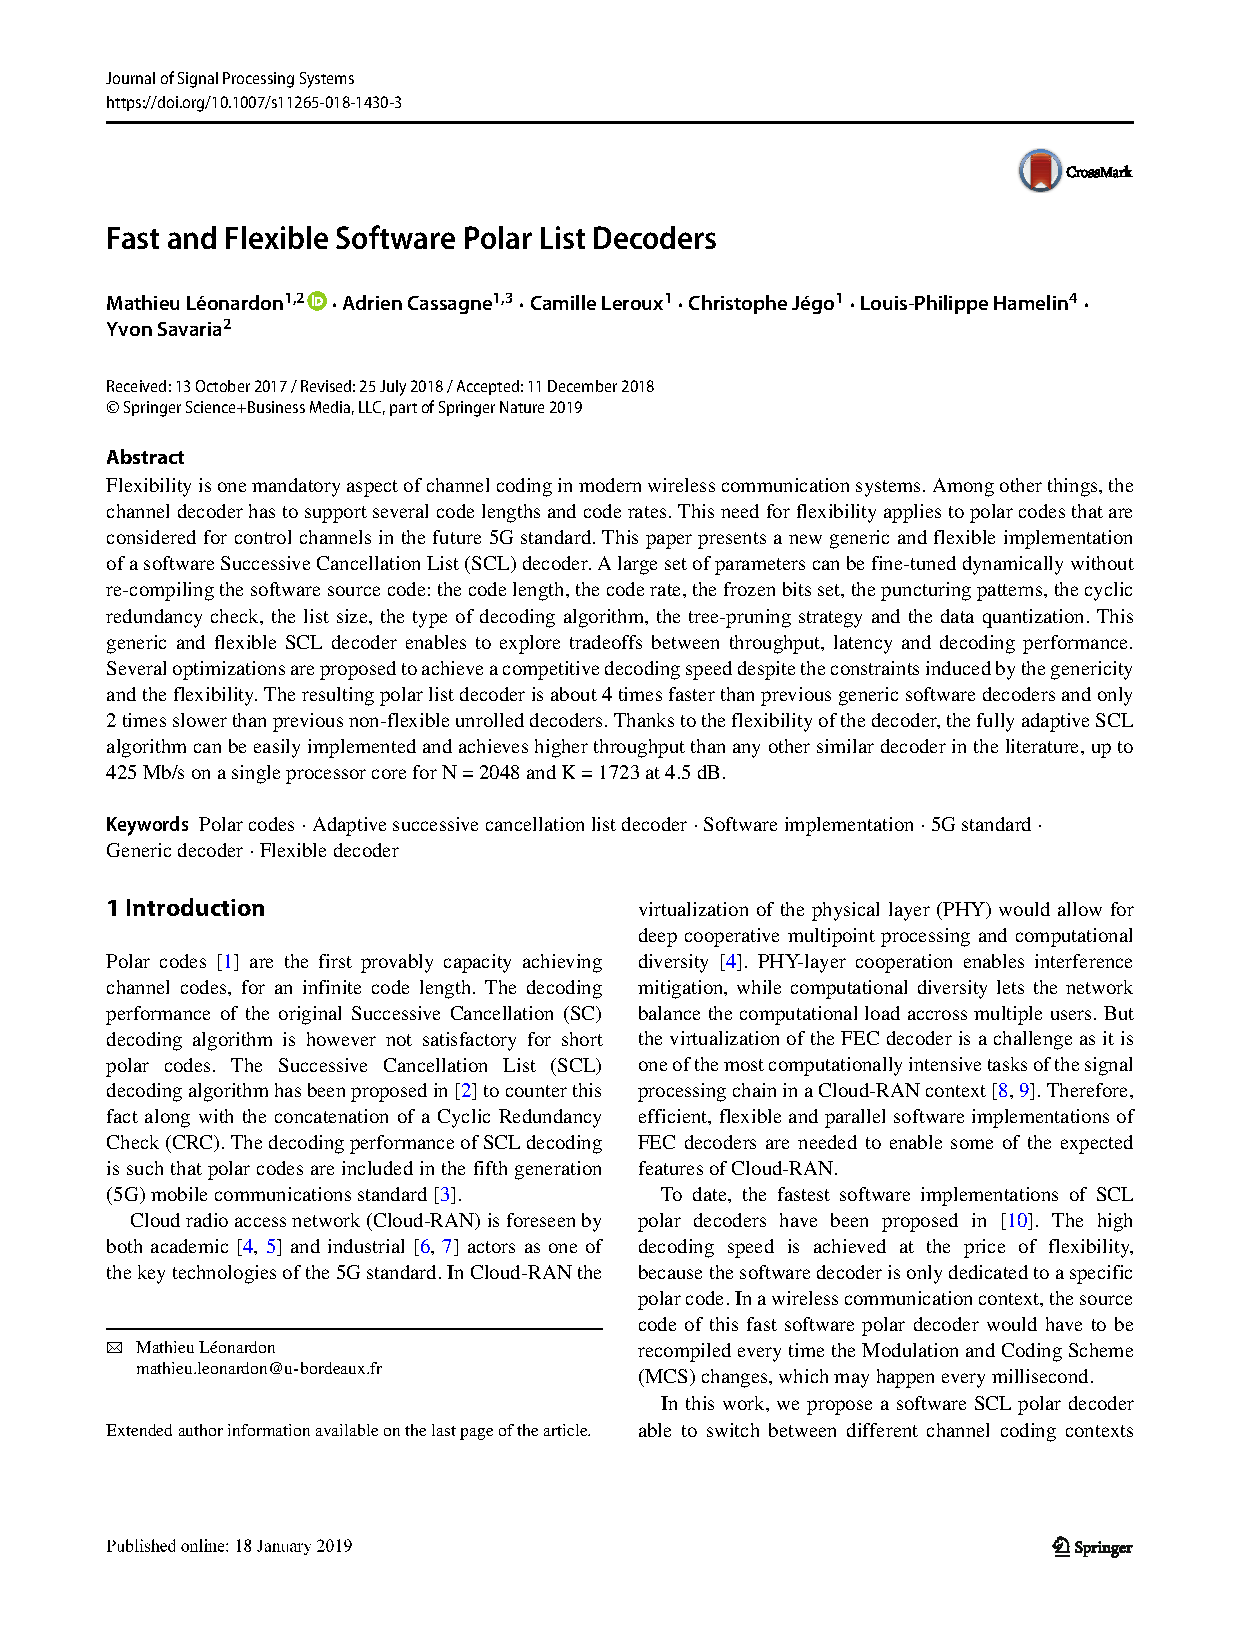
\includepdf[pages=1,pagecommand={\section{Articles}\vspace{1cm}\subsection{Fast and Flexible Software Polar List Decoders}},width=\paperwidth, offset=80 -160]{pieces/article_fast_list.pdf}
\includepdf[pages=2-,pagecommand={},width=\paperwidth, offset=80 -40]{pieces/article_fast_list.pdf}

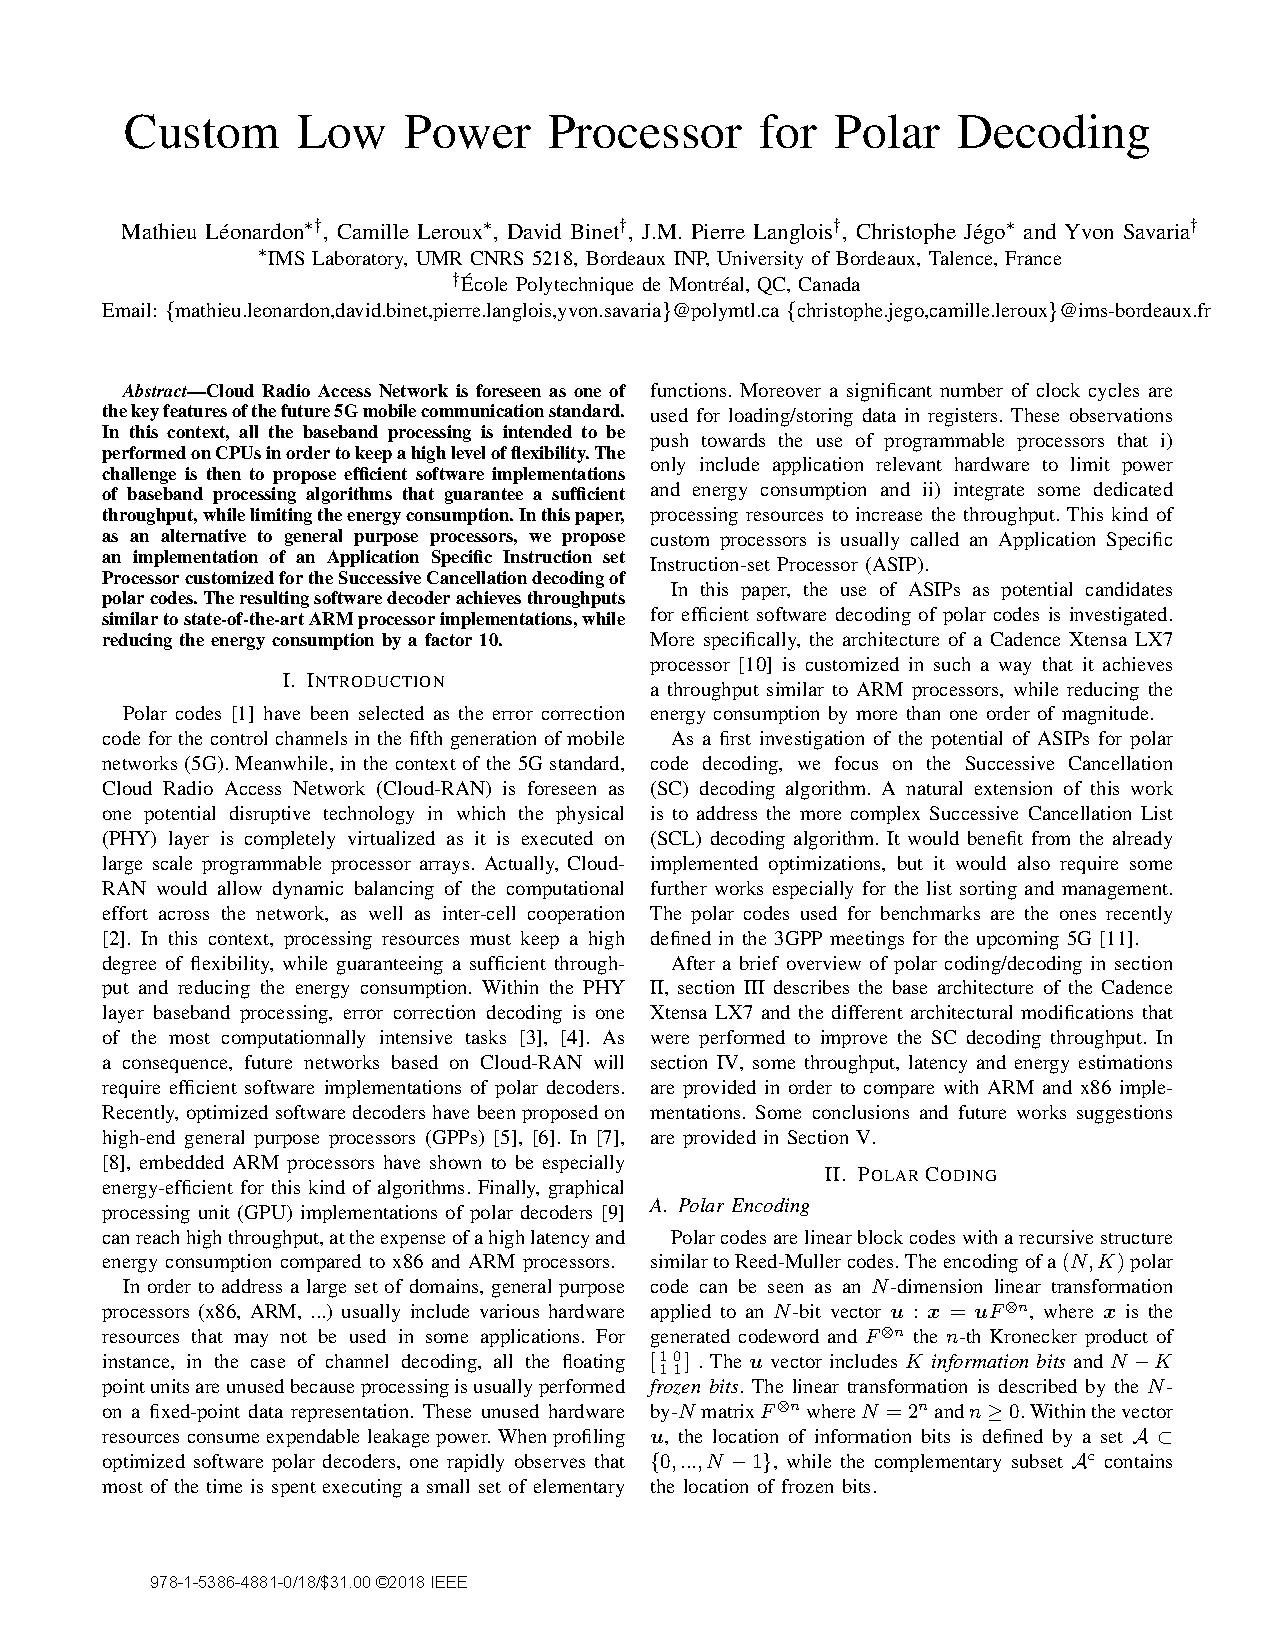
\includepdf[pages=1,pagecommand={\subsection{Custom Low Power Processors for Polar Decoding}},width=\paperwidth, offset=80 -100]{pieces/article_custom.pdf}
\includepdf[pages=2-,pagecommand={},width=\paperwidth, offset=80 -40]{pieces/article_custom.pdf}

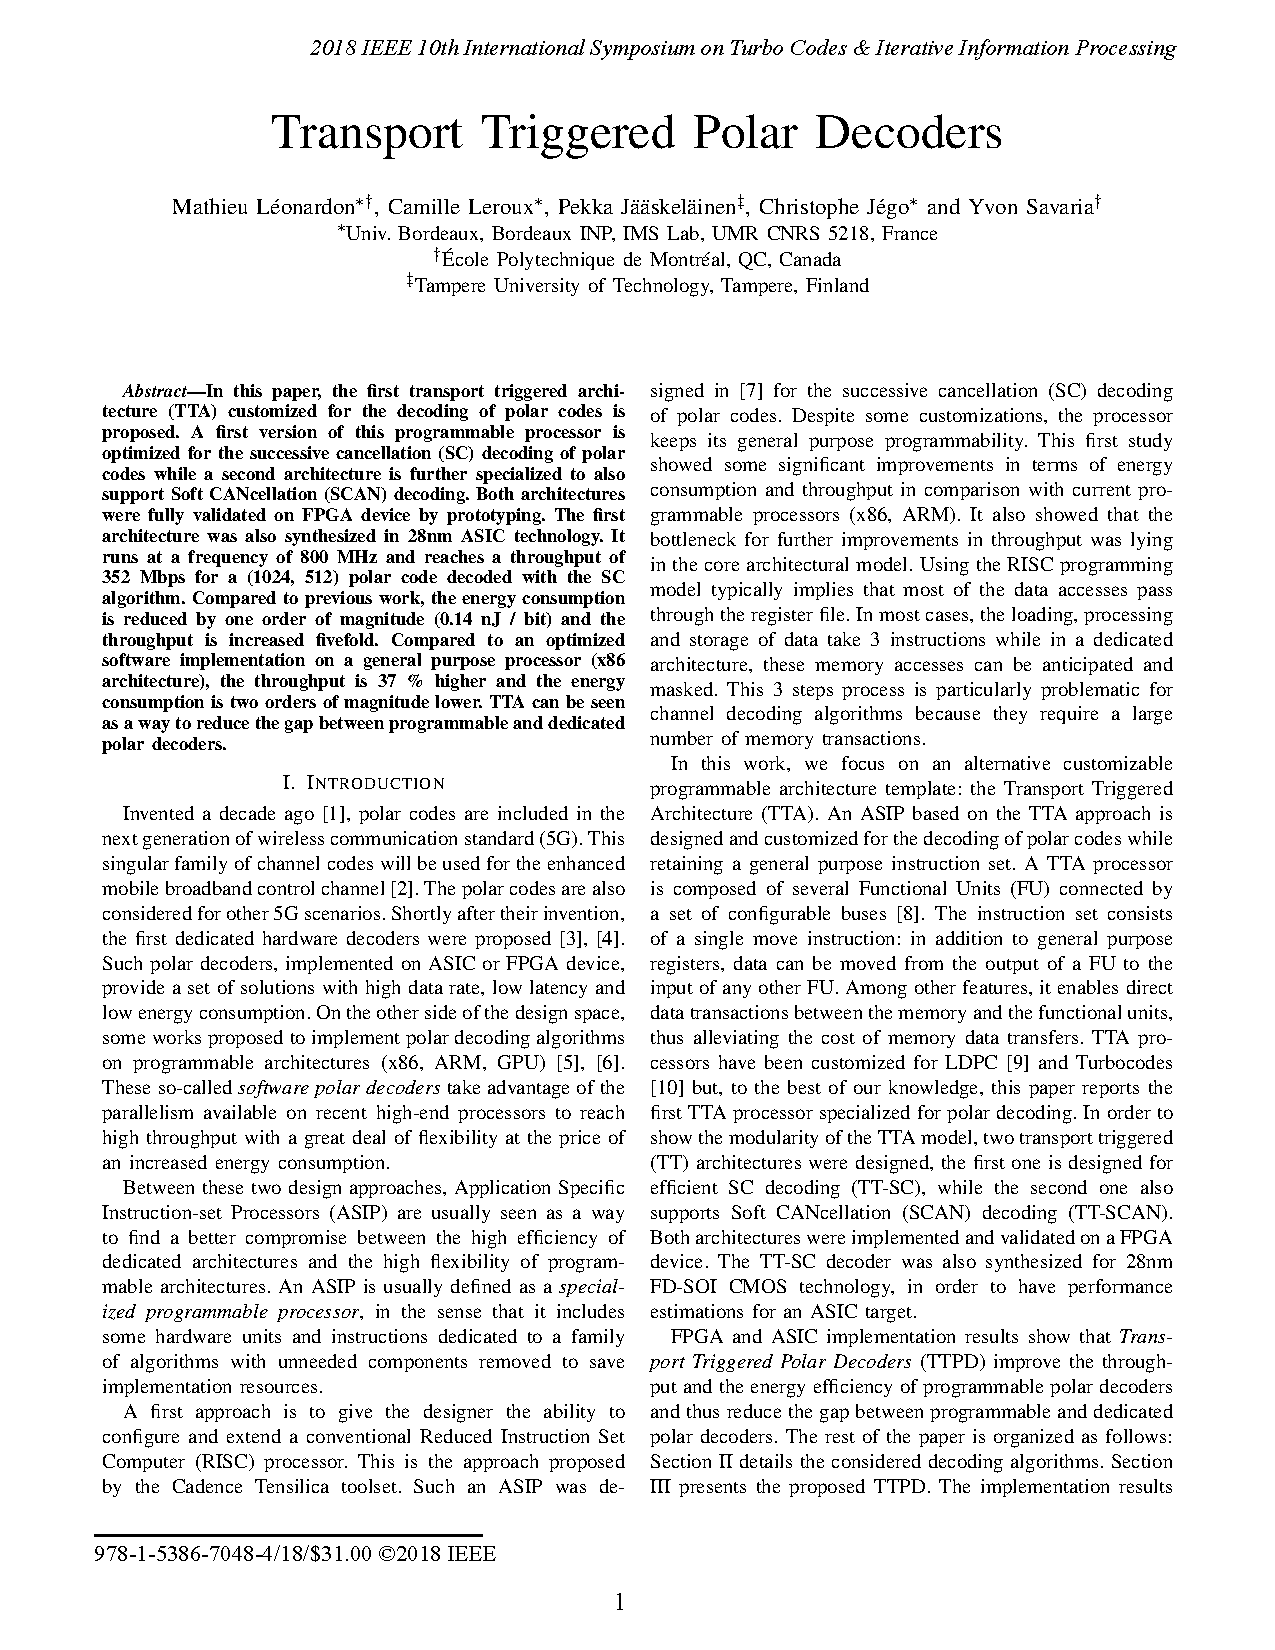
\includepdf[pages=1,pagecommand={\subsection{Transport Triggered Polar Decoders}},width=\paperwidth, offset=80 -140]{pieces/article_ttpd.pdf}
\includepdf[pages=2-,pagecommand={},width=\paperwidth, offset=80 -40]{pieces/article_ttpd.pdf}


% Rapport de soutenance

\includepdf[pages=1,pagecommand={\section{Rapports de th�se}\vspace{1cm}\subsection{Rapport de soutenance}},width=\textwidth, offset=80 -100]{pieces/rapport_soutenance.pdf}

\includepdf[pages=2-,pagecommand={},width=\textwidth, offset=80 -40]{pieces/rapport_soutenance.pdf}

% Rapport Amer

\includepdf[pages=1,pagecommand={\subsection{Rapport - Amer Baghdadi}},width=\textwidth, offset=80 -100]{pieces/rapport_amer_baghdadi.pdf}

\includepdf[pages=2-,pagecommand={},width=\textwidth, offset=80 -40]{pieces/rapport_amer_baghdadi.pdf}

% Rapport Emmanuel

\includepdf[pages=1,pagecommand={\subsection{Rapport - Emmanuel Casseau}},width=\textwidth, offset=80 -100]{pieces/rapport_emmanuel_casseau.pdf}

\includepdf[pages=2-,pagecommand={},width=\textwidth, offset=80 -40]{pieces/rapport_emmanuel_casseau.pdf}



\section{Pi�ce d'identit�}
\vspace*{2.7cm}
\begin{center}
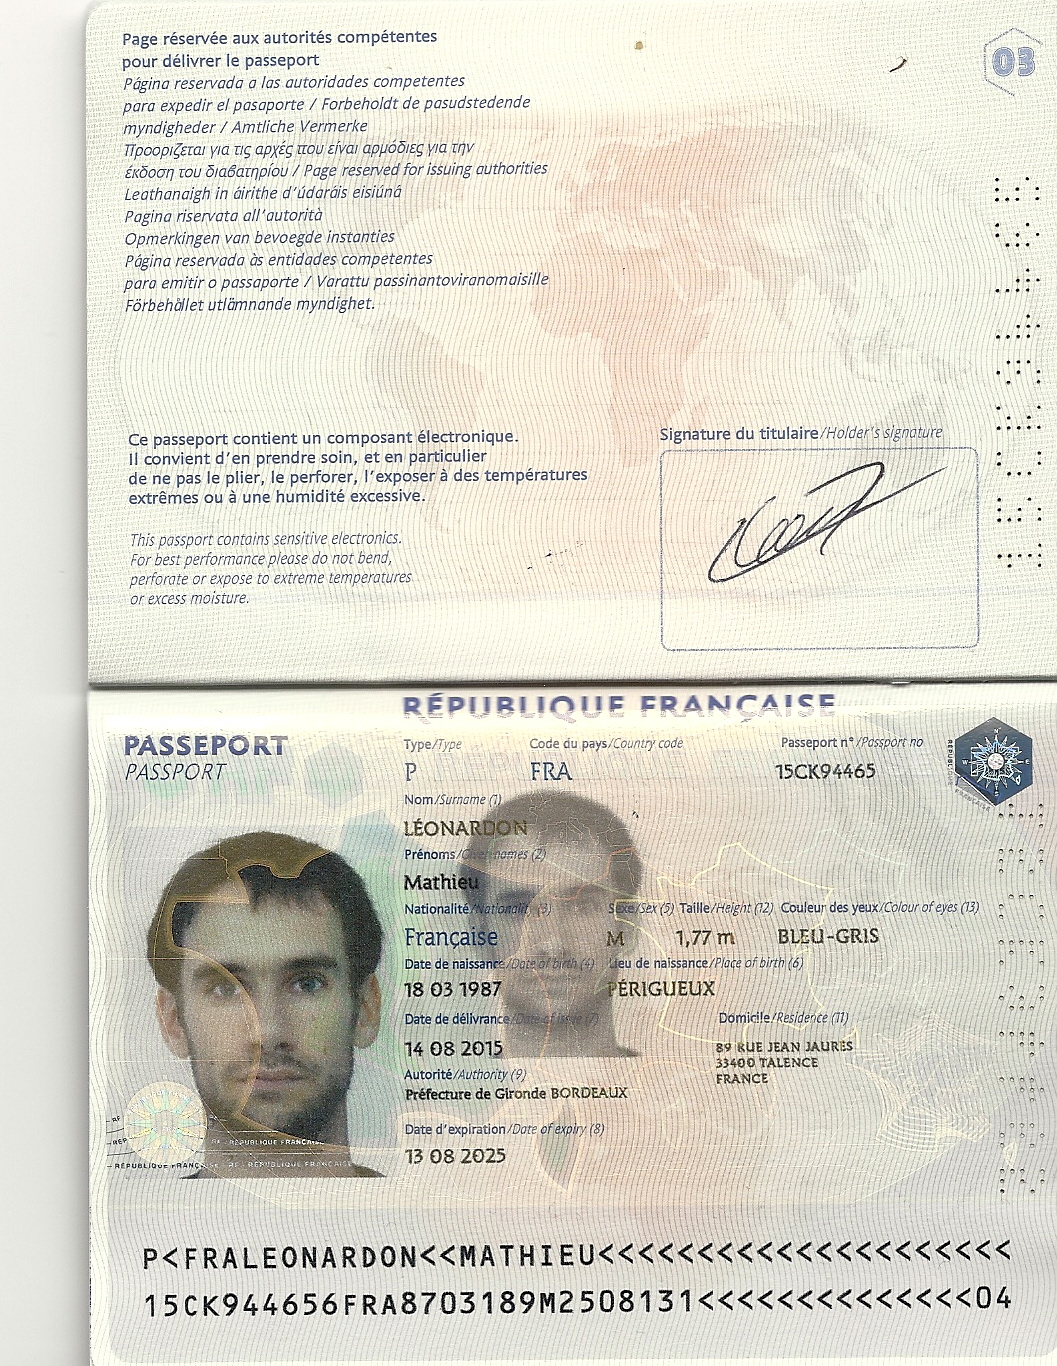
\includegraphics{pieces/passeport.jpg}
\end{center}

\newpage

\includepdf[pages=-,pagecommand={\section{Dipl\^ome de Doctorat}},width=\textwidth, offset=80 -80]{pieces/Diplome.pdf}

\end{document}
